\section{Software Development}
Software development has become more complex over the years. Today software is dependent on multiple components. More components also introduce a greater risk to software vulnerabilities. This section dives into modern software application architecture, technology stacks relevant to this thesis and attack vectors software engineers should be aware about.

\subsection{Software Architecture}
Every application has design decision in place, whether implicit or explicit. Design decisions include all the aspects of the system under development, including structure, functional behavior, nonfunctional properties, user interaction, and decisions associated to the software's implementation and deployment \cite{hasselbring2018software}. Software architectures often are described with diagrams using boxes, circles, and lines accompanied with writing.

\subsubsection{The Three-tier Architecture}

\subsection{Technology Stack}

\subsubsection{Containerization}
Docker describes a container as \say{\textit{a standard unit of software that packages up code and all its dependencies so the application runs quicly and reliably from one computing environment to another}} \cite{docker_what_container}. For many years, Linux distributions have included containers. However, due to its complexity they have rarely been used. The introduction of Docker unlocked the value of Linux containers by combining an easy to use standardized packaging format. Processes that once were abstract have become comprehensible for developers and operation teams. With Docker the process of creating a distributable product for any application, deploying it at scale into any environment is no longer complex. Docker has greatly simplified the workflow and responsiveness of agile software organizations. When implemented correctly, any organization, team, developer or operation team will benefit from the use Docker \cite{matthias2015docker}.

\begin{figure}
    \centering
    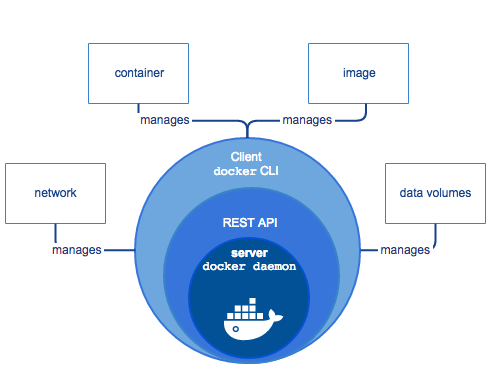
\includegraphics[width=\textwidth]{../../img/chapter_2/docker.png}
    \caption{Docker Overview}
    \label{fig:docker-overview}
\end{figure}

\subsubsection{NoSQL Databases}

\subsubsection{Application Programming Interface}

\subsubsection{The Client}

\subsection{Software Attack Vectors}

\subsection{The Software Development Life Cycle}
The SDLC plays an essential role for software engineers since it assists in defining the foundation to develop software. Even as early as the 1950s there was the need to develop methodologies for software development in order to accelerate software development. Although the complexity of software has increased, the procedure of the development life cycle should in essence stay the same whilst the implementation to each project should be tailored respectively. In practice, two important questions arise in software development \cite{langer2012guide}:
\begin{enumerate}
    \item Is the problem identified correctly?
    \item What is the proper software solution?
\end{enumerate}
The SDLC ensures that complex reliable software can be designed and developed cost-effective within the given time. Often this process is described as the SDLC model \cite{S_2017}. 

\subsubsection{Software Development Life Cycle Models}
In 1956, the first definite representation of an SDLC model was introduced by Herbert Benington. He introduced the waterfall model that describes software development as a cascading waterfall, that flows from top to bottom as seen in Figure \ref{fig:sdlc-waterfall}. This framework for software development introduced several advantages suchlike its ease to understand. However, the waterfall model also has disadvantages. For instance, working software is not available until late during the life cycle, and it is also an inadequate model for large projects \cite{S_2017}. The models begins with an incomplete implementation of a total system followed by increased functionality and performance over time assuming that all requirements are understood properly \cite{Shah_2016}. The central question SDLC models tried to answer in the early days was how to develop software at all, and what steps would be required. Consequently, the first SDLC models were sequential models such as the waterfall model \cite{Kneuper_2017}. 

\begin{figure}
    \centering
    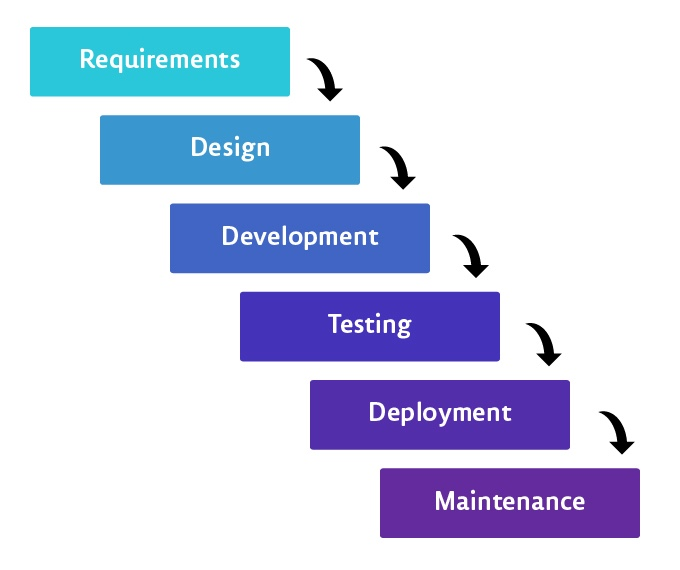
\includegraphics[width=0.5\textwidth]{../../img/chapter_2/sdlc-waterfall.jpg}
    \caption{Software Development Life Cycle - Waterfall Model}
    \label{fig:sdlc-waterfall}
\end{figure}

Today many SDLC models exist such as the Iterative Model, Spiral Model, V-Model, Big Bang Model, Agile Model, Software Prototype and Rapid Application Development Model. Unnati S. Shah et al observed that though many SDLC models exist, they are complementary, not competitive. Furthermore, they grouped all models into three broad categories; Traditional models, Agile models and Hybrid models \cite{Shah_2016}.

The objective of an SDLC model is to provide a structure for the different software development activities.  Albeit many models exist for the SDLC, it is generally divided in several phases including planning, defining requirements, design of software the architecture, development, and testing. A brief description of each phase is described below.

\paragraph{Planning}
Planning provides the foundation of every SDLC. The objective of the planning phase is to acquire the quality assurance, risk identification and feasibility report. 

\paragraph{Defining Requirements}
The next phase is centered on defining the details of the requirements gathered during the planning phase, document those and receive verification from the customer. The objective is the software development specification (SRS) document which comprises all the requirements of the product to be designed and developed.

\paragraph{Designing the Software Architecture}
Before actual development is started, the SRS is used as input to design several architectures of the software product. After reviewing the architectures the best design is selected. 

\paragraph{Development of the Product}
Based on the design of the previous phase, the actual development of the software product can begin.

\paragraph{Testing}
The final phase tests the developed software to assess whether it meets the user requirements defined in the SRS. If the tests are successful, the product can be deployed.

\subsubsection{Agile Software Development}
The "Agile Manifesto" introduced agile software development (ASD) in 2001 to the software engineering community. Described in the manifest was its purpose and principles \cite{fowler2001agile}. The four core values described in the manifesto included:

\begin{itemize}
    \item Individual and interactions over processes and tools
    \item Working software over comprehensive documentation
    \item Customer collaboration over contract negotiation
    \item Responding to change over following a plan
\end{itemize}

ASD does not assume that all requirements are clear before implementation unlike the traditional waterfall approach. As stated in the Agile Manifesto, \say{We've examined plenty of successful projects and few, if any, delivered what was planned in the beginning, yet they succeeded because the development team was agile enough to respond again and again to external changes} \cite{fowler2001agile}. Instead of trying to reject the inevitable changing nature of requirements it focuses on managing the changing nature of requirements through the SDLC as illustrated in \ref{fig:agile-dev}. Therefore, agile requires a close relationship with business expertise \cite{Shah_2016}. 

\begin{figure}
    \centering
    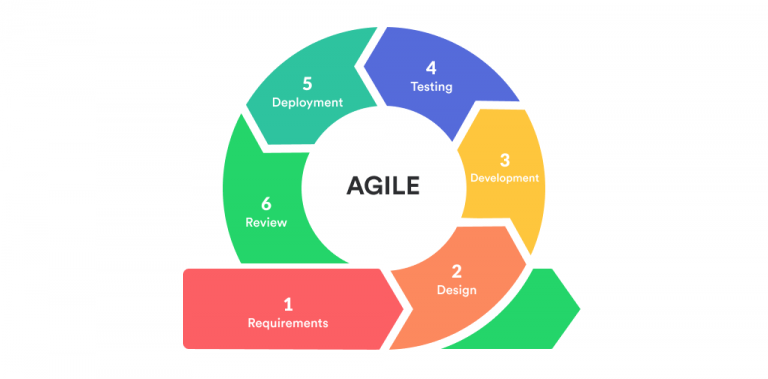
\includegraphics[width=\textwidth]{../../img/chapter_2/agile-dev.png}
    \caption{Agile Development Flow}
    \label{fig:agile-dev}
\end{figure}

\subsection{Software Security Engineering in the Software Development Life Cycle}
Secure can be defined as \say{freedom from risk and the threat of change for the worse}. From the software engineers perspective security is about engineering software such that assets are free from risk and the threat of change for the worse, or at least to the best ability. Secure programming is about designing and implementing software with the minimal amount of vulnerabilities that an attacker can exploit \cite{helfrich2019securitya}. However, modern software is complex and fragile. Despite professional engineers being capable of testing and debugging code, security is a different issue, because insecure code generally works without issues, given no attacker is exploiting the code. Software Security Engineering (SSE) introduces processes to ensure software security is ensured throughout the SDLC. 

\subsubsection{Risk Assessment}

\subsubsection{Threat Modeling}
